\chapter{CƠ SỞ LÝ THUYẾT VỀ MẠNG NƠ-RON TÍCH CHẬP VÀ MÔ HÌNH YOLO}

\section{Mạng nơ-ron tích chập}
Mạng nơ ron tích chập (Convolutional Neural Network - CNN) là một kiến trúc mạng nơ ron được sử dụng phổ biến trong lĩnh vực xử lý ảnh và nhận dạng đối tượng. Đặc điểm chính của CNN bao gồm:

\begin{itemize}
	\item Lớp tích chập (Convolutional Layer): Là lớp cốt lõi của CNN, sử dụng phép tích chập để trích xuất đặc trưng từ ảnh đầu vào. Lớp này sử dụng các bộ lọc (filter) để thực hiện phép tích chập trên ảnh và tạo ra các feature map, trong đó mỗi pixel của feature map biểu diễn mức độ kích hoạt của một đặc trưng cụ thể.
	\item Lớp gộp (Pooling Layer): Được sử dụng để giảm kích thước của feature map và giảm số lượng tham số trong mạng. Lớp gộp thường áp dụng các phép tổng hợp như lấy giá trị lớn nhất (Max Pooling) hoặc lấy giá trị trung bình (Average Pooling) trong một vùng nhất định trên feature map.
	\item Lớp kích hoạt (Activation Layer): Áp dụng một hàm kích hoạt phi tuyến (như ReLU - Rectified Linear Unit) sau lớp tích chập để tạo độ không tuyến tính và giúp mô hình học được các đặc trưng phức tạp hơn.
	\item Lớp kết nối đầy đủ (Fully Connected Layer): Là một loại lớp nơ ron truyền thống, kết nối các đặc trưng đã được trích xuất từ lớp trước với các nơ ron trong lớp này. Lớp này thường xuất ra các đầu ra cuối cùng của mạng, thường là các xác suất phân loại của các lớp đối tượng.
	\item Hàm mất mát (Loss Function): Được sử dụng để đánh giá sự khác biệt giữa kết quả dự đoán và giá trị thực tế. Các hàm mất mát phổ biến trong CNN bao gồm hàm Cross-Entropy và hàm Mean Squared Error.
	\item Tính chia sẻ tham số (Parameter Sharing): CNN sử dụng cơ chế chia sẻ tham số giữa các vùng không gian trong ảnh để giảm số lượng tham số cần học. Thay vì học các trọng số riêng cho mỗi vùng của ảnh, CNN chia sẻ các trọng số giữa các vùng có cùng đặc trưng.
	\item Kiến trúc kiểu "tầng" (Layered Architecture): CNN được tổ chức thành một chuỗi các lớp xếp chồng lên nhau, mỗi lớp đóng vai trò trong việc trích xuất và học các đặc trưng từ dữ liệu. Kiến trúc kiểu "tầng" giúp mạng học được các đặc trưng từ cấp thấp đến cấp cao, từ các nét cơ bản đến các đặc trưng phức tạp hơn.
\end{itemize}

\begin{figure}
	\centering
	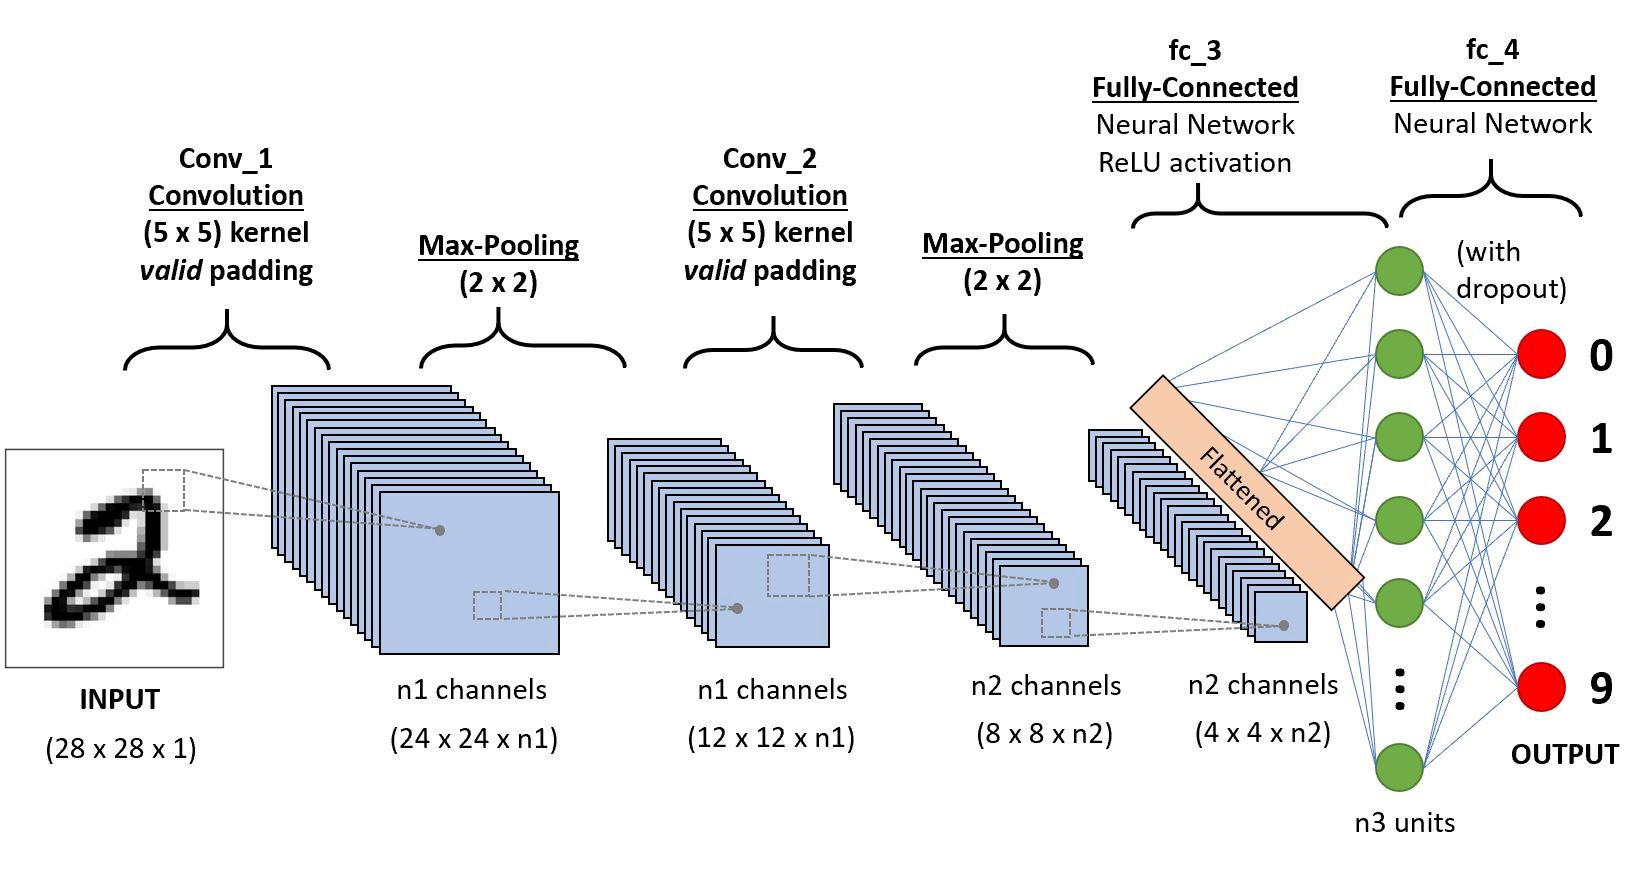
\includegraphics[width=0.9\linewidth]{images/typical-cnn.png}
	\caption{Mạng nơ-ron tích chập điển hình\cite{Ratan_2023}}
	\label{fig:typical-cnn}
\end{figure}

Tổng quan, mạng nơ ron tích chập là một kiến trúc mạng nơ ron đặc biệt được thiết kế để xử lý và trích xuất đặc trưng từ dữ liệu ảnh. Các đặc điểm của CNN như lớp tích chập, lớp gộp, lớp kích hoạt, lớp kếtnối đầy đủ và tính chia sẻ tham số giúp cho CNN có khả năng học và trích xuất các đặc trưng từ dữ liệu ảnh một cách hiệu quả. Kiến trúc kiểu "tầng" trong CNN cho phép mạng học được các đặc trưng từ cấp thấp đến cấp cao, từ các nét cơ bản đến các đặc trưng phức tạp hơn.


\subsection{Lớp tích chập}
Trong mạng CNN, lớp tích chập thực hiện áp dụng phép tích chập giữa các bộ lọc (filter) và đầu vào để tạo ra các feature map, từ đó trích xuất các đặc trưng của dữ liệu.

\begin{itemize}
    \item Bộ lọc (Filter/Kernel): Mỗi lớp tích chập bao gồm một hoặc nhiều bộ lọc (filter/kernel). Mỗi bộ lọc là một ma trận có kích thước nhỏ (thường là vuông) chứa các trọng số. Các trọng số này đại diện cho các đặc tính hoặc mẫu cụ thể mà lớp tích chập cố gắng tìm kiếm trong dữ liệu đầu vào.
    \item Phép tích chập: Lớp tích chập áp dụng phép tích chập giữa bộ lọc và đầu vào. Phép tích chập là một phép toán biểu thị sự tương quan giữa bộ lọc và một phần của đầu vào. Quá trình này di chuyển bộ lọc qua toàn bộ đầu vào bằng cách trượt nó qua tất cả các vị trí có thể trên đầu vào. Tại mỗi vị trí, phép tích chập tính toán tổng trọng số của các phần tương ứng trong bộ lọc và đầu vào.
    \item Độ dịch chuyển (Stride): Độ dịch chuyển (stride) là khoảng cách giữa các vị trí liên tiếp khi thực hiện phép tích chập. Nếu stride là 1, bộ lọc sẽ di chuyển một bước một vị trí trong mỗi lần tính toán. Nếu stride lớn hơn 1, bộ lọc sẽ di chuyển nhanh hơn và kích thước của các feature map sẽ nhỏ hơn so với đầu vào.
    \item Lề (Padding): Đôi khi, lề (padding) được sử dụng để bảo toàn kích thước của đầu vào khi thực hiện phép tích chập. Lề là việc thêm các giá trị 0 xung quanh đầu vào ban đầu để tạo ra một khung (border) xung quanh nó. Lề có thể giúp duy trì kích thước của dữ liệu trong suốt quá trình tích chập, đồng thời giảm thiểu việc mất mát thông tin ở cạnh biên.
    \item Hàm kích hoạt: Sau khi tính toán phép tích chập, một hàm kích hoạt phi tuyến tính (như hàm ReLU, Sigmoid, hoặc Tanh) thường được áp dụng cho mỗi phần tử trong feature map. Hàm kích hoạt giúp giới hạn đầu ra của lớp tích chập và tạo độ không tuyến tính trong mô hình.
    \item Đầu ra: Kết quả của lớp tích chập là các feature map, trong đó mỗi feature map biểu diễn mức độ kích hoạt của một đặc trưng cụ thể trong dữ liệu đầu vào. Số lượng feature map được tạo ra phụ thuộc vào số lượng bộ lọc sử dụng trong lớp tích chập.
\end{itemize}

Lớp tích chập được sử dụng trong mạng CNN để trích xuất các đặc trưng cấp thấp (như cơ bản như cạnh, góc, hoặc đường cong) từ dữ liệu đầu vào. Qua các lớp tích chập và các lớp kết nối đầy đủ (fully connected layers) sau đó, mạng CNN có thể học các đặc trưng ngày càng phức tạp hơn và phân loại các đối tượng trong ảnh, nhận dạng âm thanh, hoặc thực hiện nhiều tác vụ khác liên quan đến dữ liệu không gian như video hoặc dữ liệu 3D.


\subsection{Lớp gộp}
Lớp gộp (pooling layer) là một thành phần quan trọng trong mạng nơ-ron tích chập (CNN) để giảm kích thước không gian của đặc trưng và giảm độ phức tạp tính toán.

Nguyên lý hoạt động của lớp gộp như sau:

\begin{itemize}
    \item Khung gộp (Pooling window): Lớp gộp sử dụng một khung gộp (pooling window) có kích thước nhỏ để trượt qua feature map đầu vào. Khung gộp thường có kích thước vuông và di chuyển trên feature map với một stride (độ dịch chuyển) cho trước.
    \item Phép gộp (Pooling operation): Tại mỗi vị trí của khung gộp, một phép toán gộp (pooling operation) được áp dụng để giảm kích thước của đặc trưng. Có hai phép gộp phổ biến được sử dụng trong CNN:
    \begin{itemize}
        \item Max pooling: Phép gộp tối đa (max pooling) chọn giá trị lớn nhất từ khung gộp làm đại diện cho vùng đó. Nó giúp giữ lại thông tin quan trọng và đặc trưng nổi bật trong vùng đó.
        \item Average pooling: Phép gộp trung bình (average pooling) tính trung bình giá trị của khung gộp và sử dụng giá trị trung bình đó làm đại diện cho vùng đó. Phép gộp trung bình giúp giảm nhiễu và làm mờ đặc trưng.    
    \end{itemize}
    
    \item Độ dịch chuyển (Stride): Giống như lớp tích chập, lớp gộp cũng có thể sử dụng độ dịch chuyển (stride) để xác định khoảng cách di chuyển của khung gộp trên feature map. Nếu stride là 1, khung gộp sẽ di chuyển một bước một vị trí trong mỗi lần tính toán. Nếu stride lớn hơn 1, khung gộp sẽ di chuyển nhanh hơn và kích thước của feature map gộp (output feature map) sẽ nhỏ hơn so với đầu vào.
    \item Kích thước đầu ra: Kích thước của output feature map sau lớp gộp phụ thuộc vào kích thước của đầu vào, kích thước khung gộp, stride và phép gộp được sử dụng. Thông thường, lớp gộp giảm kích thước không gian của đặc trưng, giúp giảm số lượng tham số và tính toán trong mạng CNN.
\end{itemize}

Lớp gộp thường được sử dụng sau mỗi lớp tích chập trong mạng CNN để giảm kích thước không gian của đặc trưng và tổng quát hóa thông tin. Việc giảm kích thước không gian giúp giảm số lượng tham số và tính toán, đồng thời tạo ra các đặc trưng cấp cao hơn bằng cách tóm tắt thông tin từ các vùng lớn hơn của đầu vào.

Tuy nhiên, lớp gộp cũng có một nhược điểm là khiến mất mất một số thông tin chi tiết, vì chỉ giữ lại thông tin quan trọng nhất. Điều này có thể làm mất một số thông tin nhỏ nhưng quan trọng, đặc biệt đối với các bài toán yêu cầu độ chính xác cao.

\subsection{Lớp kích hoạt}
Lớp kích hoạt (activation layer) trong mạng nơ-ron là một lớp không có trọng số và thường được đặt sau mỗi lớp tích chập hoặc lớp kết nối đầy đủ (fully connected layer) trong mạng nơ-ron.

Nguyên lý hoạt động của lớp kích hoạt như sau:

\begin{itemize}
    \item Đầu vào: Lớp kích hoạt nhận đầu vào từ lớp trước đó trong mạng nơ-ron. Đầu vào có thể là một tensor hoặc một ma trận, tùy thuộc vào kiến trúc của mạng nơ-ron.
    \item Hàm kích hoạt: Lớp kích hoạt áp dụng một hàm kích hoạt phi tuyến tính lên đầu vào. Hàm kích hoạt này thường được chọn để giới hạn đầu ra và tạo độ không tuyến tính cho mạng nơ-ron. Một số hàm kích hoạt phổ biến bao gồm:
    \begin{itemize}
        \item Hàm ReLU (Rectified Linear Unit): $f(x) = max(0, x)$. Nó giữ nguyên giá trị không âm và bỏ qua các giá trị âm.
        \item Hàm Sigmoid: $f(x) = \frac{1}{(1 + exp(-x))}$. Nó chuyển đổi giá trị đầu vào thành một phạm vi từ $0$ đến $1$, thường được sử dụng trong các bài toán phân loại nhị phân.
        \item Hàm Tanh: $f(x) = \frac{(exp(x) - exp(-x))}{(exp(x) + exp(-x))}$. Tương tự như hàm sigmoid, nhưng đầu ra nằm trong khoảng từ $-1$ đến $1$.
        \item Hàm Softmax: $f(x_i) = \frac{exp(x_i)}{sum(exp(x_j))}$, với $i$ là chỉ số của đầu ra và $j$ là chỉ số của tất cả các đầu ra. Hàm softmax thường được sử dụng trong bài toán phân loại đa lớp để chuyển đổi đầu vào thành các xác suất phân loại.
    
    \end{itemize}
    \item Đầu ra: Kết quả của lớp kích hoạt là đầu ra của lớp này, được truyền tới lớp tiếp theo của mạng nơ-ron.
\end{itemize}
    
Lớp kích hoạt chủ yếu được sử dụng để tạo độ không tuyến tính trong mạng nơ-ron và giúp mô hình học được các đặc trưng phức tạp và biểu diễn các mô hình quan hệ phi tuyến. Nó cũng giúp giới hạn đầu ra trong một phạm vi nhất định và tạo ra các đầu ra dễ hiểu và dễ xử lý cho các lớp tiếp theo.

Các hàm kích hoạt và vị trí của lớp kích hoạt trong mạng nơ-ron có thể được điều chỉnh tùy thuộc vào bài toán cụ thể và kiến trúc mạng nơ-ron.

\subsection{Lớp kết nối đầy đủ}
Lớp kết nối đầy đủ (fully connected layer), còn được gọi là lớp đầu ra (output layer) trong mạng nơ-ron, là một trong những loại lớp quan trọng trong kiến trúc mạng nơ-ron truyền thẳng (feedforward neural networks).

Nguyên tắc hoạt động của lớp kết nối đầy đủ như sau:

\begin{itemize}
    \item Đầu vào: Lớp kết nối đầy đủ nhận đầu vào từ lớp trước đó trong mạng nơ-ron. Đầu vào thường là một vector hoặc một tensor được duỗi thành một vector.
    \item Trọng số và độ lệch: Mỗi nút trong lớp kết nối đầy đủ kết nối với tất cả các nút trong lớp trước đó thông qua một trọng số (weight) tương ứng. Mỗi kết nối có một trọng số riêng. Ngoài ra, mỗi nút cũng có một độ lệch (bias) tương ứng.
    \item Tính toán: Đầu vào của mỗi nút trong lớp kết nối đầy đủ được nhân với trọng số tương ứng và cộng với độ lệch. Sau đó, kết quả được đưa qua một hàm kích hoạt phi tuyến tính (như hàm ReLU, sigmoid, tanh) để tạo ra đầu ra của nút đó.
    \item Đầu ra: Kết quả tính toán của mỗi nút trong lớp kết nối đầy đủ là đầu ra của lớp này. Đầu ra có thể là một vector hoặc một tensor tùy thuộc vào số lượng nút trong lớp.
\end{itemize}

Lớp kết nối đầy đủ thường được sử dụng trong các mạng nơ-ron truyền thẳng để tạo ra đầu ra cuối cùng của mạng. Nó giúp mô hình học được các mối quan hệ phức tạp giữa đầu vào và đầu ra. Các lớp kết nối đầy đủ thường được sử dụng trong các bài toán như phân loại ảnh, nhận dạng giọng nói, bài toán dự báo, và nhiều bài toán khác.

Một số kiến trúc mạng nơ-ron sử dụng nhiều lớp kết nối đầy đủ liên tiếp nhau để tạo thành một mạng nơ-ron sâu (deep neural network). Trong các mạng nơ-ron sâu, thông qua việc kết hợp nhiều lớp kết nối đầy đủ với các hàm kích hoạt phi tuyến tính, mô hình có khả năng học được các đặc trưng phức tạp và biểu diễn các mô hình quan hệ phi tuyến giữa đầu vào và đầu ra.

\subsection{Mạng tích chập toàn phần (Fully Convolution Network)}
\subsection{Mạng Residual (ResNet)}

\subsection{Thuật toán chuẩn hóa theo lô (Batch norm)}

\subsection{Nguyên lý hoạt động của mạng nơ-ron tích chập}

\subsection{Huấn luyện và tinh chỉnh mạng nơ-ron tích chập}
\subsubsection{Hàm mất mát}
Hàm mất mát (loss function), còn được gọi là hàm chi phí (cost function) hoặc hàm mục tiêu (objective function), là một hàm số đo lường mức độ sai khác giữa các dự đoán của mạng nơ-ron và giá trị thực tế (ground truth) trong quá trình huấn luyện mạng nơ-ron.

Mục tiêu của một mạng nơ-ron trong quá trình huấn luyện là tối thiểu hóa giá trị của hàm mất mát. Điều này đồng nghĩa với việc mô hình càng tiến gần đến dự đoán chính xác, giá trị của hàm mất mát càng nhỏ.

Cách lựa chọn hàm mất mát phụ thuộc vào loại bài toán. Dưới đây là một số hàm mất mát phổ biến được sử dụng trong các bài toán phổ biến:

\begin{itemize}
    \item Hàm mất mát bình phương trung bình (Mean Squared Error, MSE): Hàm MSE tính toán sai khác bình phương trung bình giữa dự đoán và giá trị thực tế. Nó thường được sử dụng trong các bài toán hồi quy (regression).
    \item Hàm mất mát chéo-entropy nhị phân (Binary Cross-Entropy Loss): Hàm mất mát này thường được sử dụng trong các bài toán phân loại nhị phân, trong đó mô hình cần dự đoán một trong hai lớp. Nó đo lường sai khác giữa xác suất dự đoán và xác suất thực tế.
    \item Hàm mất mát chéo-entropy đa lớp (Categorical Cross-Entropy Loss): Hàm mất mát này phổ biến trong các bài toán phân loại đa lớp, trong đó mô hình cần dự đoán một trong nhiều lớp. Nó tính toán sai khác giữa phân phối xác suất dự đoán và phân phối xác suất thực tế.
    \item Hàm mất mát log-likelihood (Log-Likelihood Loss): Hàm mất mát này thường được sử dụng trong các mô hình xác suất như mạng nơ-ron hồi quy và mạng nơ-ron sinh. Nó đo lường sự khác biệt giữa phân phối xác suất dự đoán và phân phối xác suất thực tế dưới dạng log-likelihood.
    \item Hàm mất mát đánh giá phân phối (Kullback-Leibler Divergence Loss): Hàm mất mát này đo lường sự khác biệt giữa hai phân phối xác suất. Nó thường được sử dụng trong các mô hình sinh như mạng nơ-ron sinh đối nghịch tạo (Generative Adversarial Networks - GANs).
\end{itemize}

Các hàm mất mát khác cũng có thể được sử dụng tùy thuộc vào bài toán cụ thể và yêu cầu của mô hình. Việc lựa chọn hàm mất mát phù hợp là một phần quan trọng trong việc huấn luyện mạng nơ-ron để đạt được kết quả tốt.


\subsubsection{Thuật toán lan truyền ngược}
\subsubsection{Huấn luyện mạng nơ-ron tích chập}

Các bước huấn luyện mạng nơ-ron tích chập bao gồm:

\begin{itemize}
    \item Chuẩn bị dữ liệu: Thu thập và tiền xử lý dữ liệu huấn luyện. Điều này bao gồm việc chia dữ liệu thành các tập huấn luyện, kiểm tra và xác nhận. Ngoài ra, cần thực hiện các bước tiền xử lý như chuẩn hóa dữ liệu, cắt tỉa hoặc thay đổi kích thước ảnh.
    \item Xây dựng kiến trúc mạng: Xác định kiến trúc của mạng nơ-ron tích chập. Kiến trúc CNN thông thường bao gồm các lớp tích chập (convolutional layers), lớp gộp (pooling layers), lớp kích hoạt (activation layers) và lớp kết nối đầy đủ (fully connected layers). Kiến trúc cụ thể sẽ phụ thuộc vào bài toán và yêu cầu.
    \item Khởi tạo tham số: Khởi tạo trọng số và độ lệch của mạng nơ-ron. Có thể sử dụng các phương pháp khởi tạo ngẫu nhiên hoặc khởi tạo trước (pre-initialized) từ các mô hình đã được huấn luyện trước.
    \item Lan truyền thuận (Forward propagation): Thực hiện lan truyền thuận để tính toán đầu ra của mạng nơ-ron dựa trên đầu vào. Lan truyền thuận trong CNN bao gồm các phép tích chập, phép gộp và các hàm kích hoạt.
    \item Tính toán hàm mất mát (Loss computation): Tính toán giá trị hàm mất mát dựa trên đầu ra của mạng nơ-ron và giá trị thực tế.
    \item Lan truyền ngược (Backpropagation): Tính toán đạo hàm của hàm mất mát theo các tham số của mạng nơ-ron. Sử dụng thuật toán lan truyền ngược để lan truyền đạo hàm từ lớp cuối cùng đến lớp đầu tiên của mạng.
    \item Cập nhật tham số: Sử dụng một thuật toán tối ưu hóa (như gradient descent) để cập nhật các trọng số và độ lệch của mạng dựa trên đạo hàm tính được trong quá trình lan truyền ngược.
    \item Lặp lại quá trình: Lặp lại các bước trên với các mini-batch khác nhau của dữ liệu huấn luyện cho đến khi đạt được tiêu chí dừng (như số lượng epoch hoặc đạt được độ chính xác mong muốn trên tập kiểm tra).
    \item Đánh giá mô hình: Đánh giá mô hình được huấn luyện bằng cách đo lường độ chính xác và các phương pháp đánh giá khác trên tập kiểm tra hoặc tập xác nhận.
    \item Fine-tuning và kiểm tra: Tinh chỉnh mô hình, tăng cường dữ liệu, và thử nghiệm trên các tập dữ liệu mới để đảm bảo tính tổng quát và hiệu suất của mạng.
\end{itemize}

\subsubsection{Đánh giá hiệu suất của mạng nơ-ron tích chập}
Trong mạng nơ-ron tích chập (CNN), có một số thông số quan trọng được sử dụng để đánh giá hiệu suất của mô hình:
\begin{itemize}
    \item Accuracy (Độ chính xác): Đây là tỷ lệ phần trăm của số lượng dự đoán chính xác trên tổng số lượng dự đoán. Độ chính xác được tính bằng tỉ lệ giữa lượng dự đoán chính xác và tổng số lượng dự đoán.
    \item Precision (Độ chính xác dương tính): Precision đo lường tỷ lệ giữa số lượng dự đoán dương tính chính xác và tổng số lượng dự đoán dương tính. Precision là tỉ lệ giữa số lượng dự đoán "đúng" chính xác và tổng số lượng dự đoán "đúng".
    \item Recall (Độ nhớ tìm kiếm): Recall, còn được gọi là độ nhạy (sensitivity), đo lường tỷ lệ giữa số lượng dự đoán dương tính chính xác và tổng số lượng thực tế dương tính. Recall là tỉ lệ giữa số lượng dự đoán "đúng" chính xác và tổng số lượng dự đoán "đúng" thực tế.
    \item F1-score: F1-score là một đánh giá tổng hợp, kết hợp giữa precision và recall. Nó đo lường sự cân bằng giữa độ chính xác dương tính và độ nhạy. F1-score được tính bằng công thức: $\frac{2 * (Precision * Recall)}{(Precision + Recall)}$.
    \item mAP (mean Average Precision): mAP là một phép đo tổng hợp để đánh giá hiệu suất của mô hình trong bài toán phát hiện đối tượng. Nó tính toán trung bình của các giá trị Average Precision (AP) cho từng lớp đối tượng. Average Precision là một số đo cho biết khả năng mô hình tìm kiếm và định vị chính xác các đối tượng. mAP là một chỉ số tổng quát cho hiệu suất của mô hình trên toàn bộ các lớp đối tượng.
\end{itemize}

\subsubsection{Tinh chỉnh mạng nơ-ron tích chập}

Tùy vào mỗi bài toán, để có được kết quả tốt hơn, mạng nơ-ron tích chập có thể được tối ưu bằng một số phương pháp và kỹ thuật sau đây:

\begin{itemize}
    \item Tăng cường dữ liệu (Data augmentation): Sử dụng các phép biến đổi dữ liệu như xoay, phóng to, thu nhỏ, lật ngang, lật dọc, cắt tỉa và thay đổi độ sáng để tạo ra các phiên bản mới của dữ liệu huấn luyện. Điều này giúp mô hình học được các đặc trưng phổ quát hơn và tăng khả năng tổng quát hóa.
    \item Regularization: Sử dụng các kỹ thuật chính quy hóa như L1 hoặc L2 regularization để giảm overfitting và tăng tính tổng quát của mô hình. Các phương pháp như Dropout hoặc Batch Normalization cũng có thể được áp dụng để kiểm soát overfitting.
    \item Tối ưu hóa tham số (Parameter optimization): Sử dụng các thuật toán tối ưu hóa như stochastic gradient descent (SGD) hoặc các biến thể của nó để điều chỉnh các tham số trong mạng nơ-ron. Các thuật toán tối ưu hóa hiện đại như Adam hoặc RMSprop cũng có thể được sử dụng để tăng tốc quá trình hội tụ và đạt kết quả tốt hơn.
    \item Kiểm tra và đánh giá (Validation and evaluation): Sử dụng tập dữ liệu kiểm tra hoặc tập xác thực (validation set) để đánh giá hiệu suất của mạng trong quá trình tinh chỉnh. Điều này giúp đánh giá tính tổng quát và tránh overfitting. Có thể thay đổi các siêu tham số (hyperparameters) của mạng như tỷ lệ học (learning rate), số lượng epoch, kích thước batch để tìm ra các thiết lập tốt nhất.
    \item Transfer learning: Sử dụng mô hình đã được huấn luyện trước (pre-trained model) trên một tác vụ liên quan và sau đó tinh chỉnh mô hình đó cho tác vụ cụ thể mà bạn quan tâm. Bằng cách sử dụng transfer learning, bạn có thể tận dụng kiến thức đã học được từ các mô hình lớn và tiết kiệm thời gian huấn luyện.
    \item Grid search và cross-validation: Sử dụng kỹ thuật grid search để tìm kiếm qua một tập hợp các siêu tham số khác nhau để tìm ra các thiết lập tốt nhất cho mạng. Kỹ thuật cross-validation cũng có thể được áp dụng để đánh giá hiệu suất của mạng trên nhiều tập dữ liệu khác nhau và tránh overfitting.
\end{itemize}


\section{Mô hình YOLO}

\subsection{Giới thiệu mô hình}

Mô hình YOLO (You Only Look Once) là một mô hình phổ biến trong lĩnh vực nhận diện đối tượng và phát hiện vị trí đối tượng trong ảnh và video. Mô hình YOLO có khả năng phân loại và định vị các đối tượng trong một khung hình duy nhất một cách nhanh chóng và chính xác.

Các đặc điểm chính của mô hình YOLO bao gồm:
\begin{itemize}
    \item Kiến trúc: Mô hình YOLO sử dụng mạng nơ-ron tích chập (CNN) để trích xuất đặc trưng từ ảnh đầu vào và dự đoán các hộp giới hạn (bounding boxes) và các lớp đối tượng tương ứng. Kiến trúc gốc của YOLO được gọi là YOLOv1 và sau đó đã có các phiên bản cải tiến như YOLOv2, YOLOv3,  YOLOv4, YOLOv5, YOLOv8, ...
    \item Grid cells: Mô hình YOLO chia ảnh thành một lưới ô vuông có kích thước cố định. Mỗi ô vuông trong lưới được gọi là một grid cell. Mỗi grid cell sẽ dự đoán một số lượng hộp giới hạn và lớp đối tượng tương ứng.
    \item Dự đoán hộp giới hạn: Mỗi grid cell trong mô hình YOLO dự đoán các hộp giới hạn bằng cách dùng các tỷ lệ (scales). Mỗi hộp giới hạn được biểu diễn bằng các thông số như tọa độ (x, y) của trung tâm, chiều rộng và chiều cao của hộp.
    \item Dự đoán lớp đối tượng: Mô hình YOLO dự đoán lớp đối tượng của mỗi hộp giới hạn bằng cách sử dụng softmax trên các điểm đặc trưng (feature points) của ảnh.
    \item Non-max suppression: Sau khi mô hình YOLO đã dự đoán các hộp giới hạn và lớp đối tượng, một quá trình gọi là non-max suppression được áp dụng để loại bỏ các hộp giới hạn trùng lặp và giữ lại các hộp giới hạn có xác suất dự đoán cao nhất.
\end{itemize}


\subsection{Kiến trúc mạng của mô hình}

Kiến trúc mạng YOLO (You Only Look Once) đã trải qua nhiều phiên bản và cải tiến, bao gồm YOLOv1, YOLOv2, YOLOv3 đến YOLOv8. Tuy nhiên, YOLO hiện nay bao gồm các thành phần chính như: Backbone, Neck và Head.

\begin{itemize}
    \item Backbone network: YOLO sử dụng một mạng nơ-ron tích chập (CNN) làm cơ sở để trích xuất đặc trưng từ ảnh. Mạng nền (backbone network) trong YOLO có thể được xây dựng bằng cách sử dụng các kiến trúc như Darknet hoặc CSPDarknet.
    \item Neck: YOLO có một phần gọi là neck (cổ), được đặt giữa backbone network và head của mô hình. Neck có nhiệm vụ kết hợp các đặc trưng từ các tầng khác nhau của feature pyramid để cung cấp thông tin phong phú hơn cho việc dự đoán đối tượng.
    \item Head: Đây là phần cuối cùng của mô hình YOLO, nơi các hộp giới hạn và lớp đối tượng được dự đoán. Head của YOLO sử dụng các lớp tích chập để dự đoán tọa độ và lớp của các hộp giới hạn. Đồng thời, YOLO sử dụng các kỹ thuật như SPP (Spatial Pyramid Pooling) và PANet (Path Aggregation Network) để cải thiện khả năng phát hiện và định vị đối tượng.
\end{itemize}

Với hàm mất mát, mô hình YOLO sử dụng một hàm mất mát kết hợp giữa các thành phần như localization loss, confidence loss và class loss. Hàm mất mát này giúp tối ưu hóa mô hình và cải thiện độ chính xác của các dự đoán.

\subsection{Đánh giá hiệu suất của mô hình}

Qua các phiên bản, mô hình YOLO ngày càng được cải thiện. Hình \ref{fig:yolov8-better} cho thấy các phiên bản YOLO ngày càng được cải thiện với lượng tham số nhỏ hơn nhanh hơn nhưng hiệu suất lại cao hơn.

\begin{figure}
    \centering
    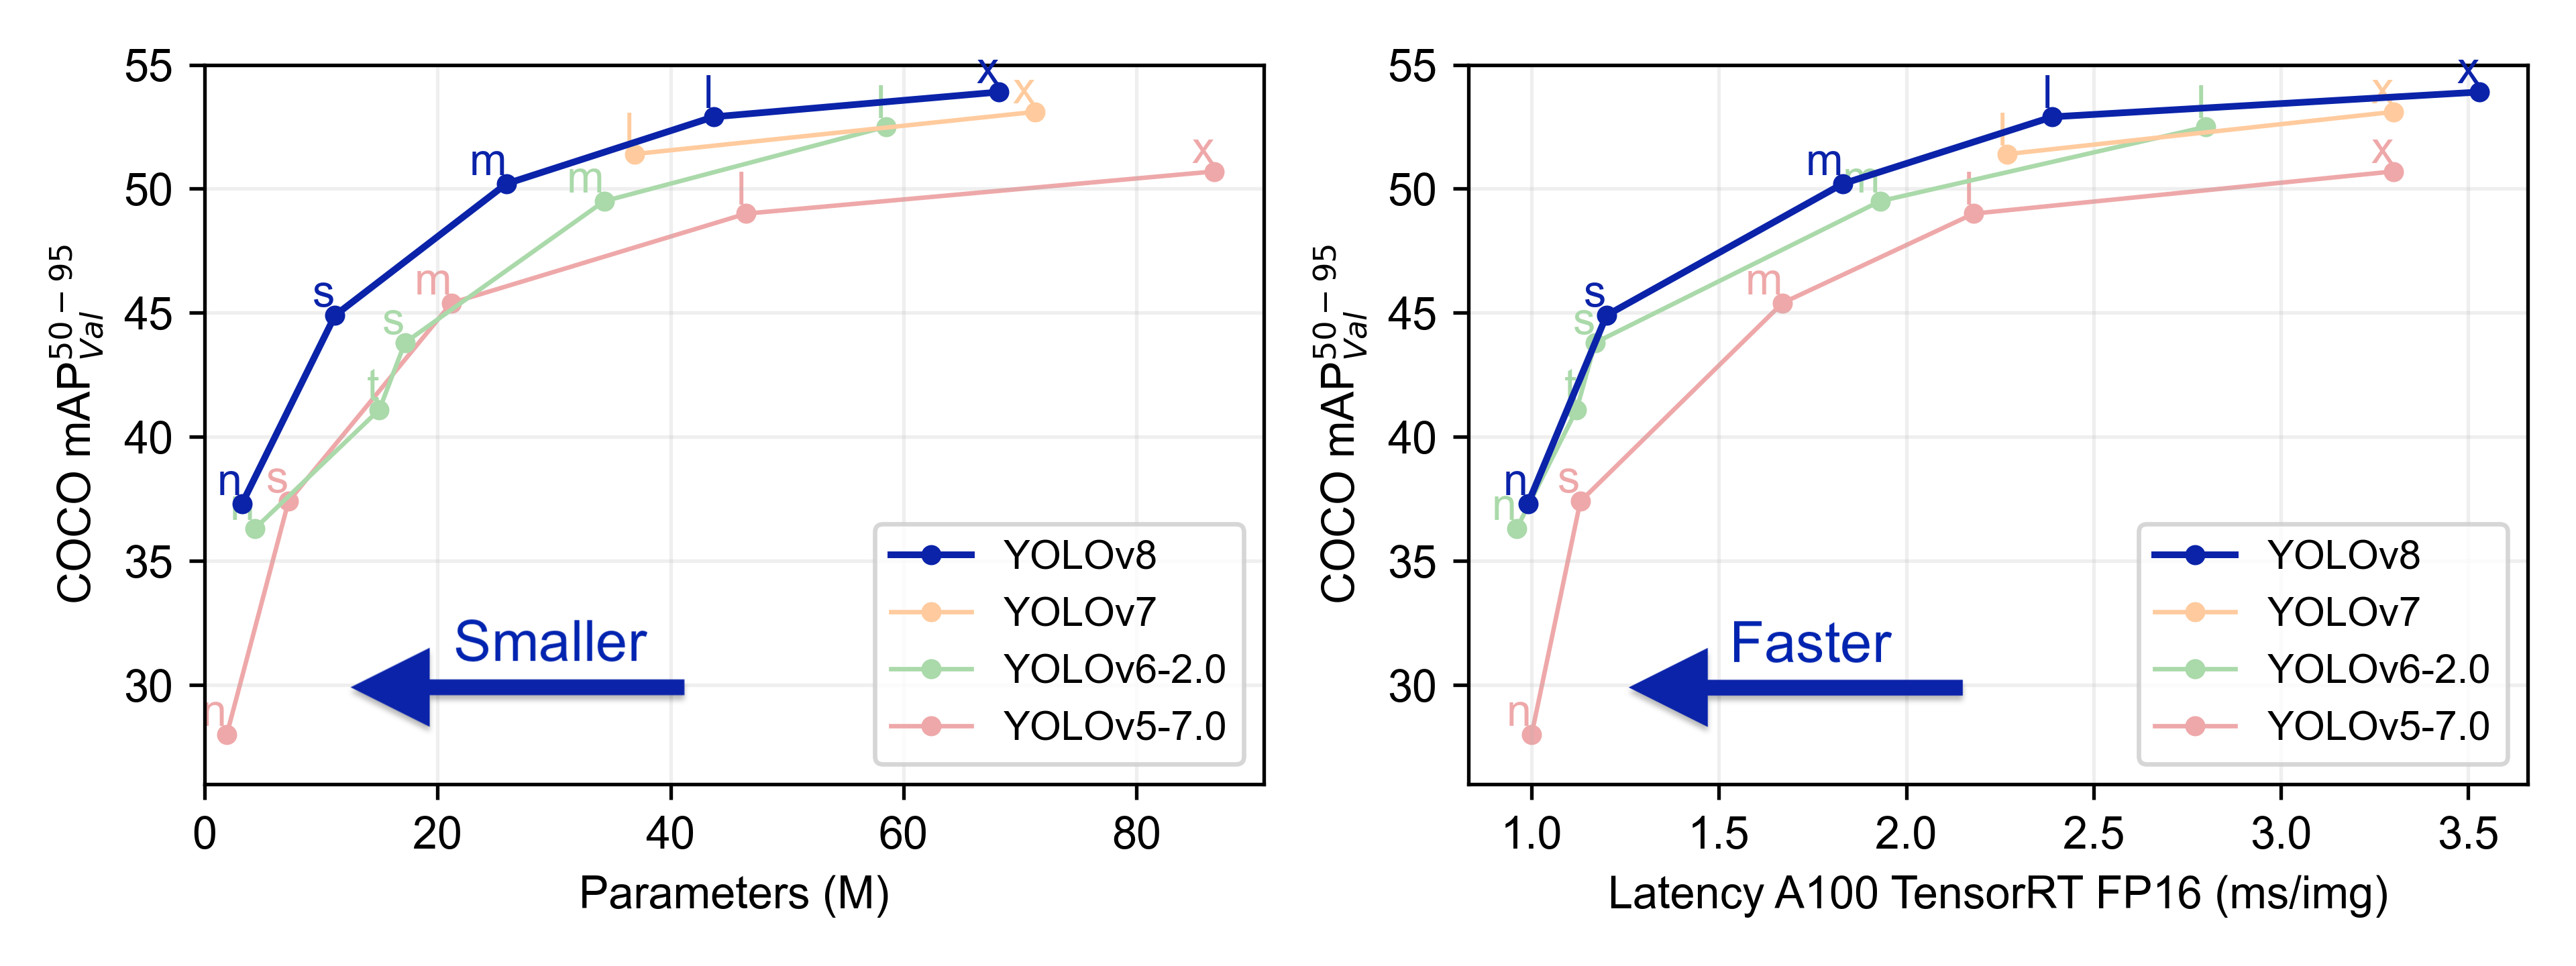
\includegraphics[width=0.75\linewidth]{images/yolov8-better.png}
    \caption{yolov8-better}
    \label{fig:yolov8-better}
\end{figure}
\subsection{So sánh YOLO và CNN trong nhận diện và phân loại ảnh}


\subsubsection{Kiến trúc mạng}
CNN là một kiến trúc mạng nơ-ron sử dụng các tầng tích chập và tầng kết nối đầy đủ để học các đặc trưng của ảnh. CNN thường sử dụng một số tầng tích chập để trích xuất đặc trưng và sau đó sử dụng các tầng kết nối đầy đủ để phân loại ảnh.

YOLO là một kiến trúc mạng nơ-ron đặc biệt được thiết kế cho việc phát hiện và định vị đối tượng trong ảnh. YOLO chia ảnh thành các lưới (grid) và dự đoán các hộp giới hạn (bounding box) và lớp đối tượng cho mỗi lưới. YOLO sử dụng một kiến trúc mạng nơ-ron tích chập để trích xuất đặc trưng và dự đoán đồng thời các hộp giới hạn và lớp đối tượng.

\subsubsection{Tốc độ}

Với CNN, việc phân loại và nhận dạng đối tượng được thực hiện trong các lớp cuối cùng của mạng. Điều này có nghĩa là CNN phải đi qua toàn bộ hình ảnh để đưa ra dự đoán, do đó, tốc độ của CNN thường chậm hơn so với YOLO.

YOLO sử dụng một phương pháp "You Only Look Once" để dự đoán đồng thời các hộp giới hạn và lớp đối tượng trên toàn bộ ảnh. Điều này giúp YOLO có tốc độ rất nhanh, vì nó không cần phải xem xét ảnh nhiều lần.

\subsubsection{Độ chính xác}

Với việc sử dụng các tầng tích chập và kết nối đầy đủ, CNN có thể học các đặc trưng phức tạp từ ảnh và đạt được độ chính xác cao trong các tác vụ phân loại và nhận dạng ảnh.

YOLO có thể cung cấp độ chính xác tương đối cao trong việc phát hiện và định vị đối tượng trong ảnh. Tuy nhiên, do việc dự đoán đồng thời trên toàn bộ ảnh, YOLO có xu hướng không chính xác hơn trong việc định vị các đối tượng nhỏ hoặc gần nhau.

\section{Nghiên cứu ứng dụng CNN và YOLO trong hệ thống theo dõi và chăm sóc nấm}

Với độ chính xác tương đối cao với tác vụ phân loại vật thể và khả năng xác định vùng bao vật thể, mô hình YOLO có thể ứng dụng trong hệ thống theo dõi và chăm sóc nấm. Bằng việc xây dựng bộ dữ liệu với các loại nấm cùng giai đoạn phát triển khác nhau, mô hình có thể cho ra biết vị trí, thời gian và giai đoạn phát triển hiện tại, giúp người nông dân đưa ra quyết định kịp thời hoặc có thể hỗ trợ điều khiển robot tự động làm việc chăm sóc hay chuẩn bị,  thu hoạch nấm.

\section{Hướng phát triển và nâng cao hiệu suất mô hình CNN và YOLO}

Đối với mô hình YOLOv8, mô hình có thể được điều chỉnh với các kích thước khác nhau (Hình \ref{fig:yolov8-structure}).

\begin{figure}
    \centering
    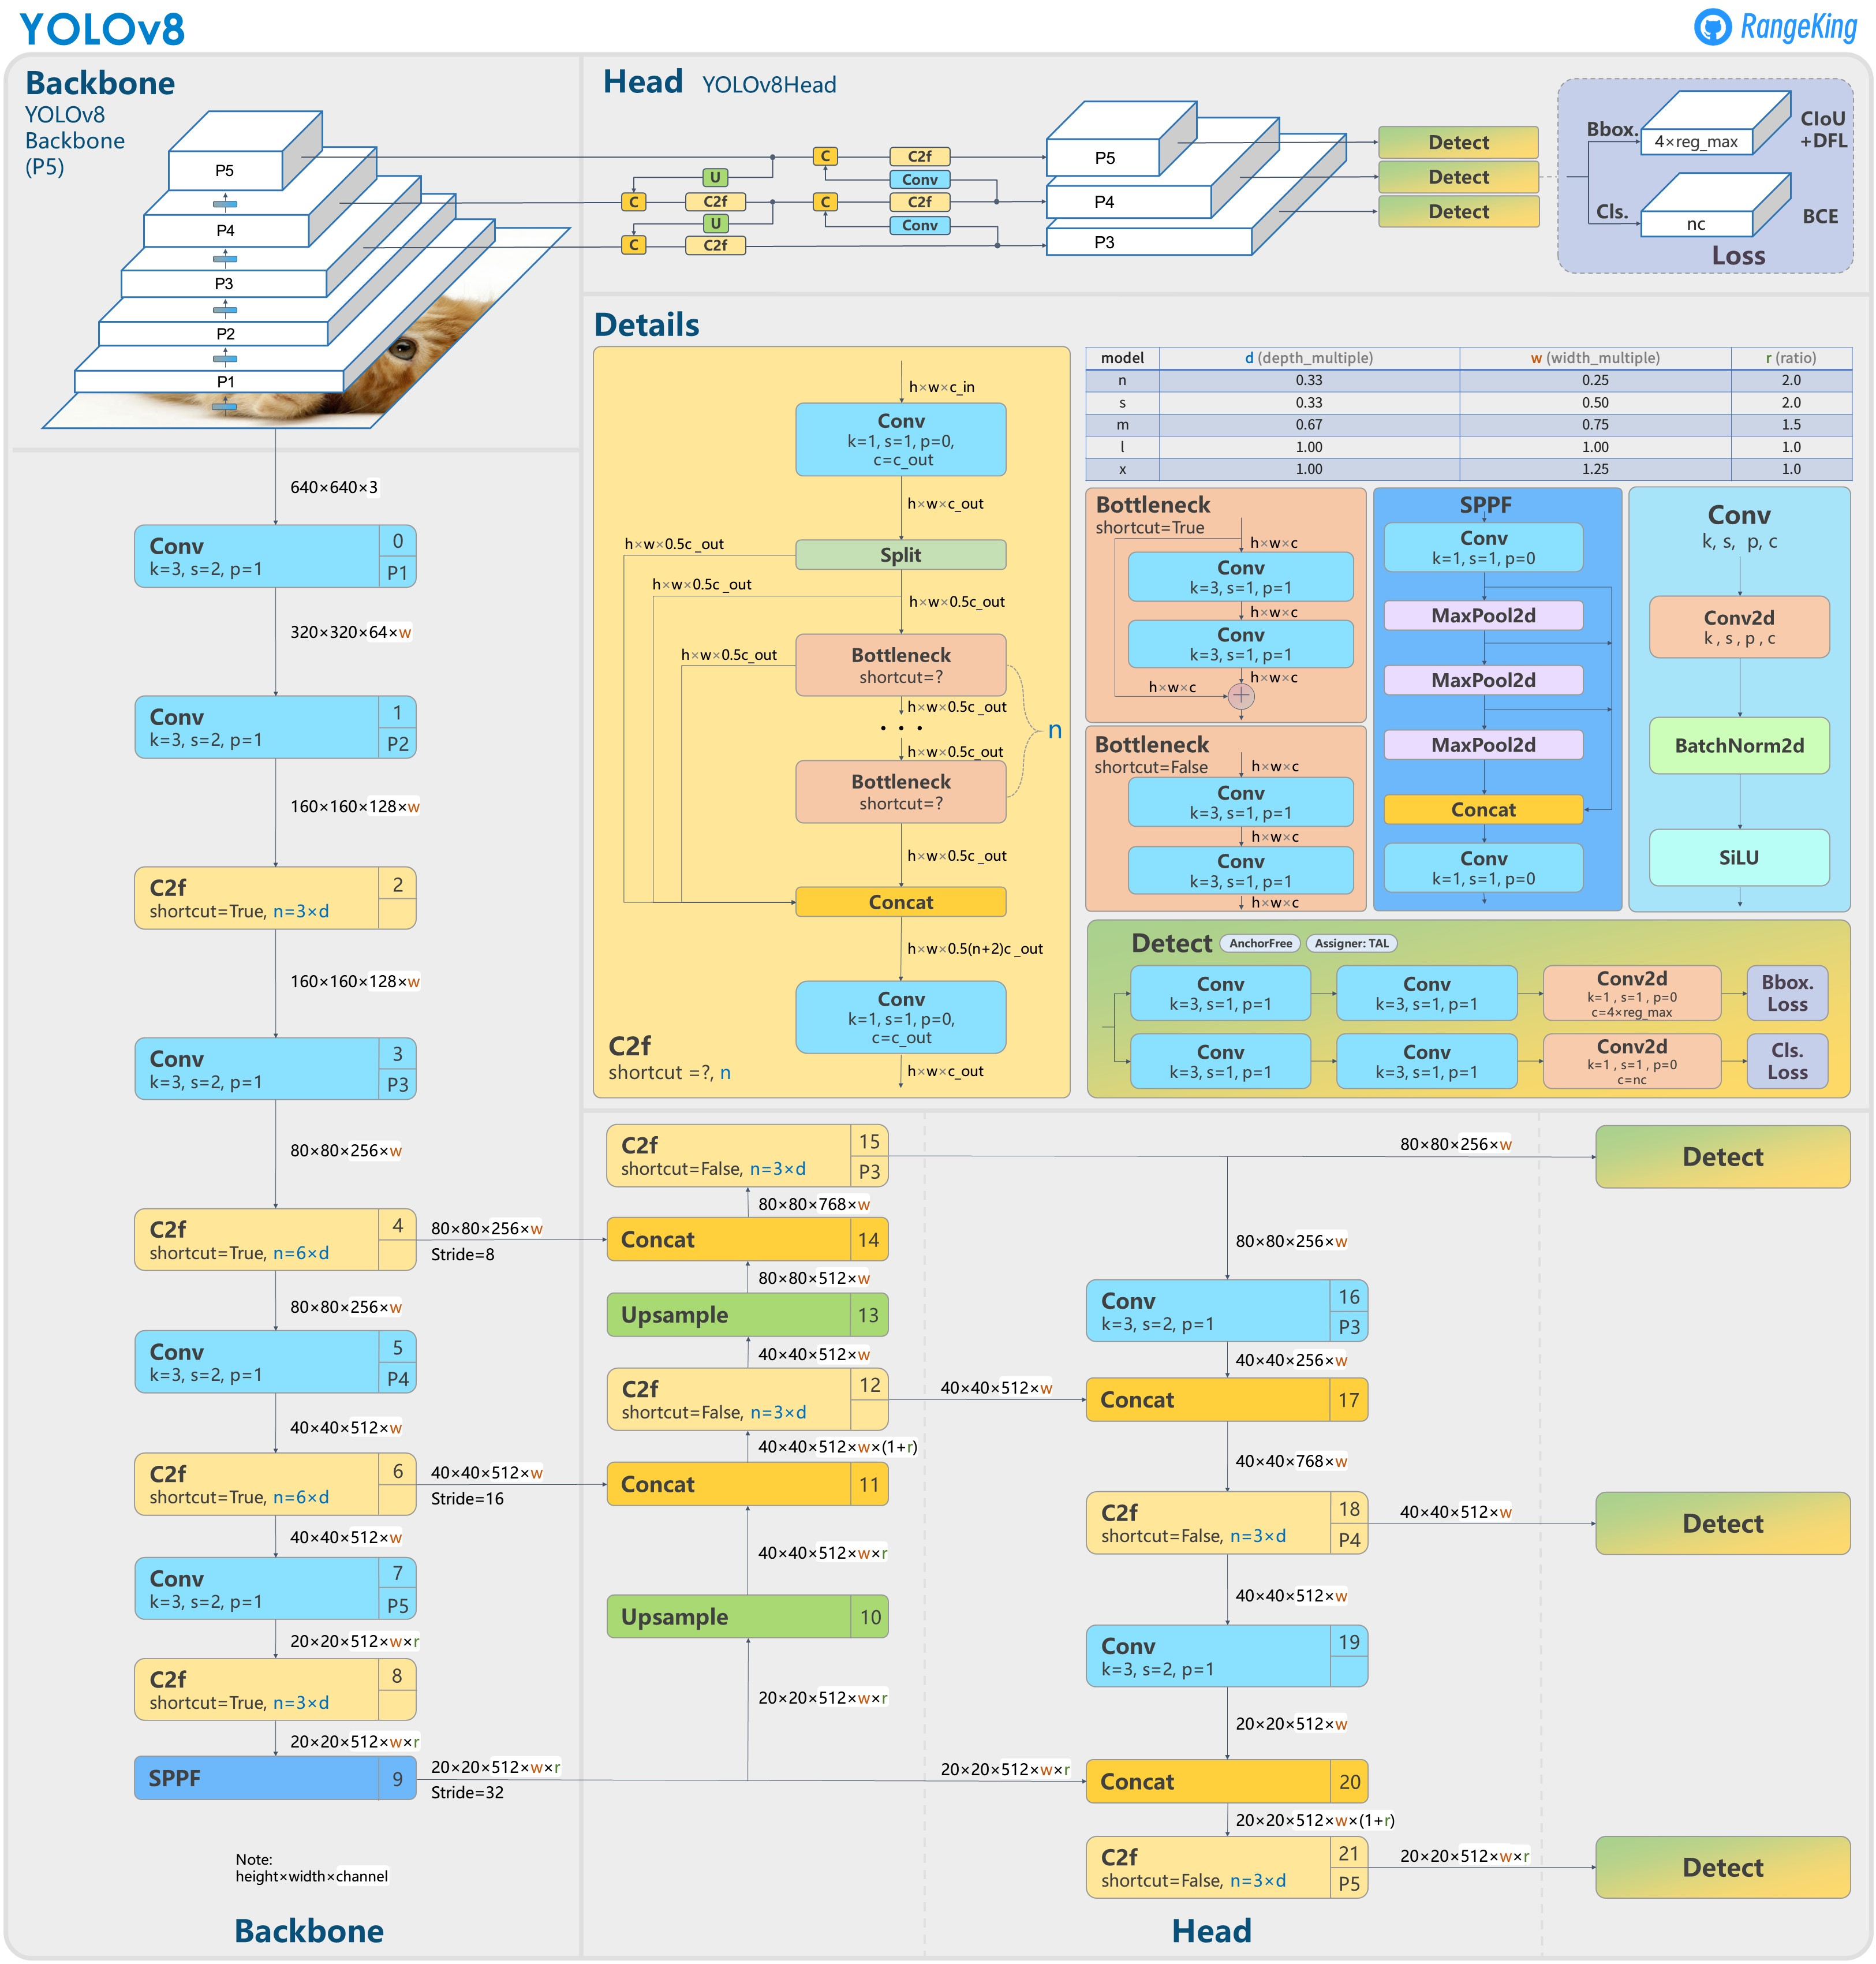
\includegraphics[width=1\linewidth]{images/yolov8-network.png}
    \caption{Cấu trúc mạng YOLOv8 và cấu hình kích thước}
    \label{fig:yolov8-structure}
\end{figure}

Với kích thước lớn - L, mô hình có khả năng học sâu hơn và đưa ra kết quả chính xác hơn. Tuy nhiên, dữ liệu đầu vào cần đa dạng và số lượng lớn hơn để có thể lấy ra những đặc trưng một cách chung nhất. Đối với số lượng mẫu nhỏ, để tránh tình trạng overfitting, kích thước nhỏ như s, n sẽ phù hợp hơn.

\section{Tổng kết chương}


Chương 2 tập trung nghiên cứu ứng dụng của mạng nơ-ron tích chập và mô hình YOLO trong hệ thống theo dõi và chăm sóc nấm.

Trước tiên, mạng nơ-ron tích chập là một mô hình học sâu được thiết kế đặc biệt cho việc xử lý dữ liệu hình ảnh. Nguyên lý hoạt động mạng dựa trên phép tích chập để lấy ra đặc trưng của ảnh, từ đó có thể phân loại ảnh vào các lớp khác nhau.

Tiếp theo, YOLO là một mô hình phát hiện và định vị đối tượng trong ảnh. Với việc chia ảnh thành các ô lưới và dự đoán hộp giới hạn và xác suất cho các đối tượng trong mỗi ô lưới, YOLO mang lại khả năng phát hiện đối tượng nhanh chóng và chính xác.

Cuối cùng là khả năng áp dụng YOLO vào hệ thống giám sát và chăm sóc nấm. Bằng việc phát hiện giai đoạn phát triển và vị trí của nấm, các công việc phân tích, chăm sóc có thể được thực hiện kịp thời. Ngoài ra, chương 2 còn để cập đến hướng phát triển và nâng cao hiệu suất của mô hình CNN và YOLO.

Như vậy, có thể thấy rằng CNN và YOLO có thể được ứng dụng trong hệ thống theo dõi và chăm sóc nấm. Sử dụng các phương pháp này, quá trình phân loại, phát hiện và định vị nấm có thể được tự động hóa, giúp tăng hiệu suất và chính xác, đồng thời giảm công sức và chi phí nhân công.
